\documentclass[12pt, a4paper]{article}
\usepackage[utf8]{inputenc}
\usepackage[russian, english]{babel}
\usepackage{indentfirst}
\usepackage[T2A]{fontenc}
\usepackage{caption}
\usepackage{listings}
\usepackage{amsmath}
\usepackage[a4paper, top=10mm, bottom=20mm]{geometry}
\usepackage{graphicx}
\usepackage[hidelinks]{hyperref}
\usepackage{tocloft}
\graphicspath{{/}}

\begin{document}

\pagenumbering{gobble}

  \begin{titlepage}
    \begin{center}
      \vspace{0.5cm}

      ДАЛЬНЕВОСТОЧНЫЙ ФЕДЕРАЛЬНЫЙ УНИВЕРСИТЕТ
      \vspace{5cm}

      {\LARGE Операционные системы\\
        \vspace{1cm}
        Реферат\\
        "Безопасность OS X"}
      \bigskip
    \end{center}

    \vspace{8cm}
    \begin{flushright}
    {\large
      Выполнил \\
      Савинов П. А\\
      Группа Б8303б}
    \end{flushright}
  \end{titlepage}

\renewcommand{\contentsname}{Содержание}
\renewcommand{\refname}{Список литературы}

\tableofcontents
\newpage

\pagenumbering{arabic}

\begin{center}
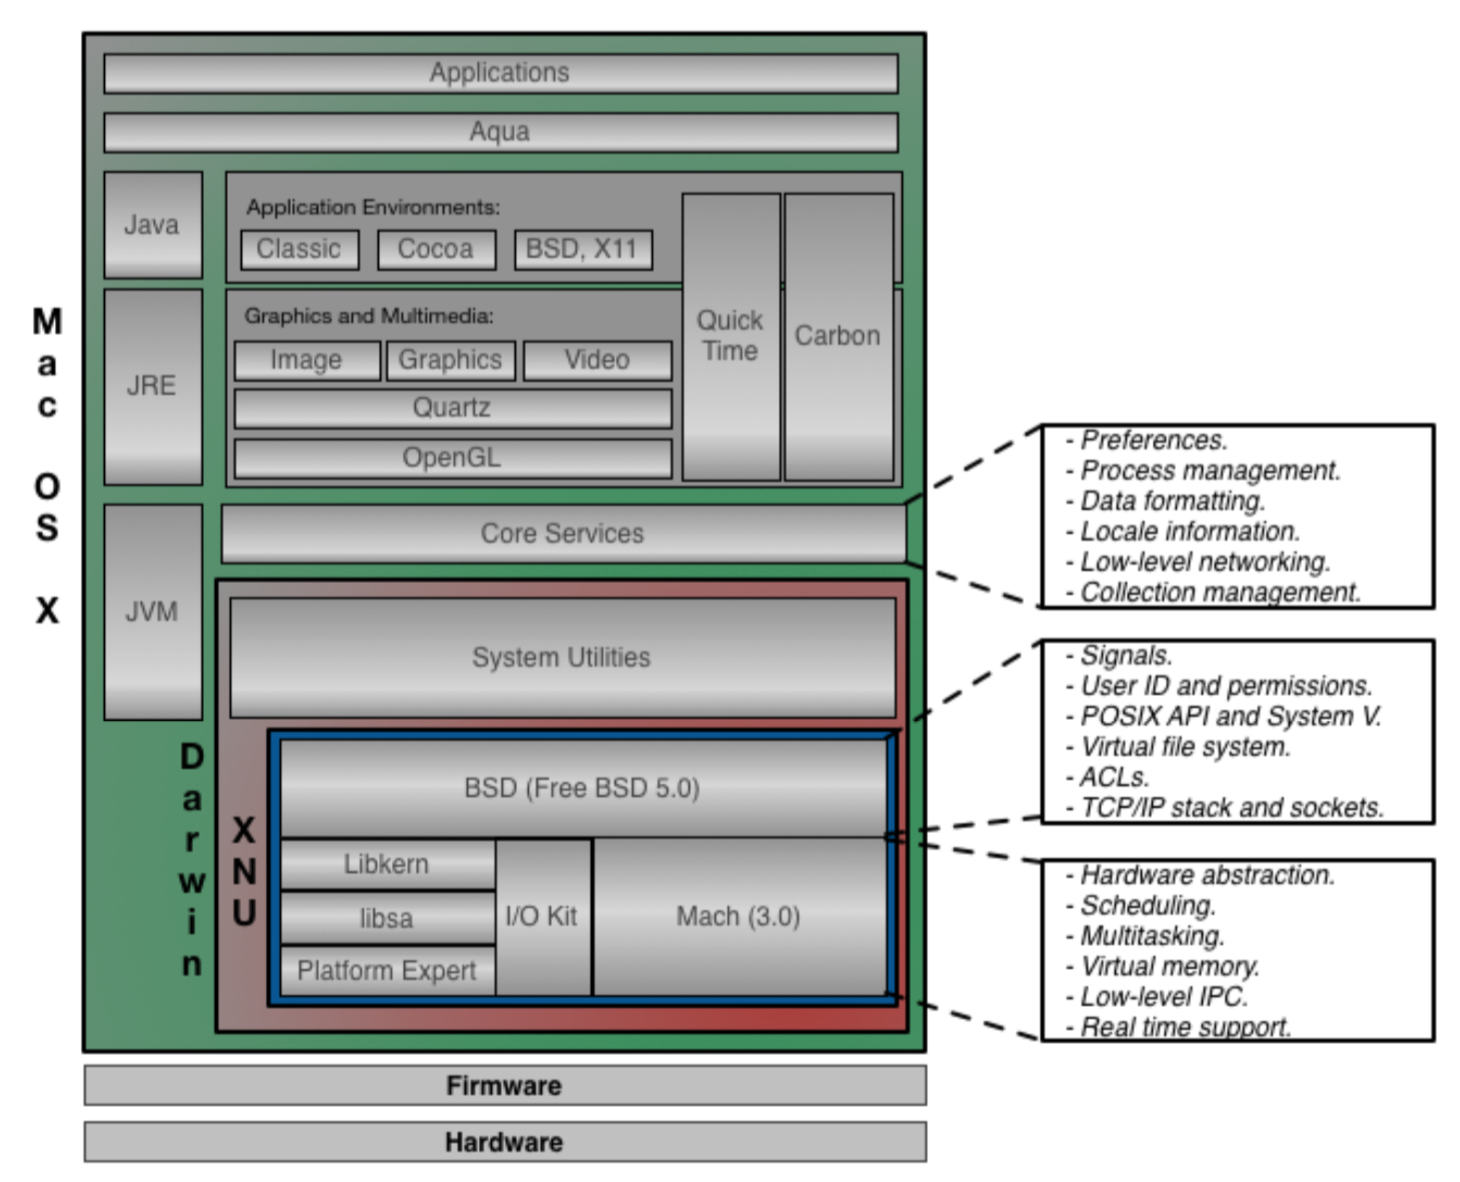
\includegraphics[width=\textwidth]{structure}
\end{center}

\section{Ядро}

Ядро Mac OS X - основано на BSD и Mach. BSD предоставляет базовую файловую систему, сетевые сервисы и реализует пользовательское и групповое разделение. BSD устанавливает ограничения доступа на основе пользователя или группы.

Mach занимается управлением памятью, контролем потоков, аппаратной абстракцией и межпроцессовым взаимодействием. Mach контролирует доступ, определяя какие задачи могут отправлять сообщения на порт Mach. (Порт Mach представляет собой задачу или какой-либо иной ресурс). Политики безопасности BSD и контроль доступа Mach составляют важную часть в безопасности Mac OS X.

\subsection{ASLR}

Address Space Layout Randomization (ASLR) - большое количество эксплойтов в малвари опирается на фиксированные местоположения хорошо известных системных функций. Чтобы подавить эти риски OS X случайным образом перемещает ядро, кексты и системные фреймворки во время загрузки системы.

\section{Права доступа}

Права доступа являются важной составляющей любой операционной системы.

В OS X права даются на уровне: папок, подпапок, файлов или приложений.

Права доступа так-же могут выдаваться на специфичные данные в файле или функции приложения.

Управление над правами доступа осуществляется на большом количестве уровней, начиная с компонентов Mach/BSD ядра, заканчивая наивысшими уровнями операционной системы. Для сетевых приложений - через сетевые протоколы.

\section{Security Framework}

Security framework в Mac OS X - реализация архитектуры CDSA. Она содержит расширяемый набор криптографических алгоритмов, для подписания кода и операций шифрования. Она так-же содержит библиотеки, которые позволяют интерпретировать сертификаты типа X.509.

CDSA код используется внутри OS X в таких приложениях, как Keychain и URL Access для защиты данных используемых для входа.

\section{Слои безопасности}

Безопасность OS X построена на нескольких слоях обороны, для максимальной безопасности.

\begin{enumerate}
  \item{Безопасные подключения | Интернет -- файрволл и фильтрация почты}
  \item{Безопасные приложения | Приложения -- шифрованные образы дисков и FileVault}
  \item{Безопасные сетевые протоколы | Сеть -- файрволл, SSL, Kerberos(Authentication)}
  \item{Сервисы безопасности | Операционная система -- keychain, POSIX/ACL(permissions)}
  \item{Secure Boot/"Lock Down" | Аппаратная часть -- firmware password utility}
\end{enumerate}

\section{Keychain}

Keychain используется для хранения ключей, сертификатов, паролей и других данных, помещенных в него пользователем. Внутренности шифруются.

Может быть разблокирован, после аутентификации пользователя(пароль, цифровой токен, смарт-карту, или биометрический сканнер). Приложения, так-же могут хранить свои данные в Keychain, соотвественно пользователь будет получать уведомление об этом(реализовано через системное API).

\section{Приложения}

В OS X существуют два типа приложений: исторические бинарники, как в *nix, и собственный формат .app.

В первом случае, дистрибуция весьма ограничена. Нет централизованного, официального репозитория(или даже пакетного менеджера), но есть подобное от сообщества, MacPorts или Brew. В этом случае применяются всё то-же, что можно сказать про любой *nix.

Второй тип, распространяется изначально, только через App Store, то есть приложение должно быть подписано ключом(private/public key) - code signing, который выдан разработчику Apple, эта функциональность именуется Gatekeeper. В настройках системы возможно отключить такое поведение, тогда возможно устанавливать в том числе и распространяемые не через App Store приложения.

\section{Sandbox}

Sandbox включается по решению разработчика, чтобы ограничить доступ извне к его приложению. Например, mDNSResponder использует подобную стратегию, а так-же паттерн pub/sub (по факту он даже не знает о своих подписчиках)

Стандартные приложения вроде Safari, Mail и т.д. работают внутри Sandbox'а.

Sandbox на уровне ядра. Его стратегия следующая:

\begin{enumerate}
  \item{Позволяет описать, как приложение взаимодействует с системой, система даёт приложению права}
  \item{Позволяет пользователю неявно давать приложению дополнительные права, например диалог Открыть/Сохранить, drag&drop и другие похожие пользовательские действия}
\end{enumerate}

\subsection{Mandatory access controls}

Sandbox'ы построены на низкоуровневном механизме контроя доступа в подсистеме ядра - kauth. kauth идентифицирует валидного actor'а(обычно процесс) с помощью его данных. Затем, он опрашивает одного или более слушателей, чтобы определить может ли данный actor выполнить данное действие в заданной области(авторизационном домене). Только первоначальный(дефолтный) слушатель может разрешить запрос; последующие могут только отклонить или отложить. Если все слушатели откладывают, kauth отклоняет запрос.

\subsection{Entitlements}

Sandbox'ы собирают эти низкоуровневые действия в отдельные entitlement'ы, которые приложение должно явно запросить добавляя соотвествующий ключ в список свойств(файл plist) в свой application bundle(.app).

Могут контролировать доступ к:

\begin{enumerate}
  \item{Вся файловая система}
  \item{Отдельные папки}
  \item{Сеть}
  \item{iCloud}
  \item{Hardware (например, камера или микрофон)}
  \item{Персональная информация(например, контакты)}
\end{enumerate}

Дополнительно, они могут контролировать, наследует ли процесс родительские права, а так-же могут предоставлять временные исключения на отправку/получение событий и чтение/запись файлов.

\subsection{Пользователские намерения}

Различные действия, вроде Drag&Drop файла, автоматически отслеживаются системой и система автоматически открывает брешь в Sandbox для этого конкретного файла, так что приложение сможет прочитать его, не запрашивая entitlement'ы.

\section{Файловый Карантин}

Карантин - мера безопасноти, которая помещает в карантин файлы загруженные из интернета.

Встроенные приложения, вроде Safari, iMessage, Mail будут генерировать предупреждение для пользователя, спрашивая уверен ли он, что хочет открыть файл. Так-же возможность известная, как XProtect проверяет на предмет известной малвари(насколько известно проверяет по хэшу ВСЕГО файла, база заполняется Apple), перед тем, как пользователь откроет файл.

\section{System Integrity Protection}

Одним из наибольших изменений в OS X 10.11 стало обрезание безграничных прав доступа ко всем частям системы у root пользователя, то есть наследия Unix-основанной системы. Эта возможность называется Rootless.

Защита целостности состоит из нескольких пунктов:

\begin{enumerate}
  \item{Файловая система -- системные пути не могут быть перезаписаны, даже root аккаунтом. Системные файлы могут быть изменены только процессами подписанными ключами, принадлежащими Apple. Процессы принадлежащие приложениям, должны записывать данные в места предназначенные для сторонних разработчиков}
  \item{Защита времени исполнения(Runtime) -- сторонние приложения не могут прицепляться(attach) к системным процессам. Системные исполняемые файлы могут быть изменены только установщиками или системным обновлением от Apple. Внедрение кода или runtime attachment сторонними приложения более невозможно.}
  \item{Расширения ядра -- расширения ядра(kext) должны быть подписаны валидным сертификатом Apple Developer.}
\end{enumerate}

\section{Summary}

Из коробки система имеет весьма неоптимальные настройки безопасности, но здесь хорошо подходит фраза <<Безопасность системы в руках её администратора>>.

В основном, все заявления о бесконечной безопасности это разумеется маркетинг.

Просто существуют объективные сложности при reverse engineering'е системы, а так-же информация об устройстве системы не особо распространена.

% \cite{SnowLeopardSecurityGuide}

\newpage
\addcontentsline{toc}{section}{\refname}
% \bibliographystyle{gost-styles/utf8gost71u

\bibliographystyle{utf8gost71u}

\makeatletter
\renewcommand{\@biblabel}[1]{#1}   % Заменяем библиографию с квадратных скобок на точку
\makeatother
\nocite{*}
\bibliography{bibliography}


\end{document}
